% Proposed revision based on the supplied Adam section.
% All numerical findings below are retained from that section, not recomputed.
% Existing figure/table paths and labels are preserved.
% The analytic bridge is derived under smooth full-objective assumptions.
% AUTHOR comments identify analyses that have NOT yet been performed.
% Add the BibTeX entry at the end to the main bibliography.
% The existing figure's eta*kappa label denotes the same numerical z statistic.

\section{Gradient Response and Optimizer Memory during Adam Loss Excursions}
\label{sec:adam-diagnostics}

The GD experiments distinguish local gradient reversal from the longer-term
reduction of the objective. Under Adam, a further distinction is necessary:
the current loss slope and the optimizer's update depend on different
information. We examine how changes in the raw gradient accompany the rise
and recovery of loss-defined excursions, and how the first-moment state
responds along these trajectories. The purpose is to characterize event
anatomy and its relationship to optimizer state.

Bai et al.~\cite{bai2026adaptive} identify a mechanism involving delayed
second-moment adaptation and preconditioned curvature. We relate our
projected-gradient response to their directional quantity below. The
relationship makes explicit the roles of first-moment response and
curvature variation along the realized step.

\subsection{Loss-Slope Measurements along Adam Trajectories}

Adam~\cite{kingma2014adam} transforms the raw gradient through first-
and second-moment estimates,
\begin{equation}
\begin{aligned}
m_t&=\beta_1m_{t-1}+(1-\beta_1)g_t,\\
v_t&=\beta_2v_{t-1}+(1-\beta_2)g_t^{\odot2},
\end{aligned}
\label{eq:adam-moments}
\end{equation}
with zero initial moments. Bias correction gives
$\widehat m_t=m_t/(1-\beta_1^t)$ and
$\widehat v_t=v_t/(1-\beta_2^t)$, followed by
\begin{equation}
d_t=\frac{\widehat m_t}{\sqrt{\widehat v_t}+\epsilon},
\qquad \theta_t=\theta_{t-1}-\eta d_t,
\label{eq:adam-direction}
\end{equation}
where operations are coordinatewise and
$g_t=\nabla\mathcal L(\theta_{t-1})$ in the full-objective experiments.

Although $d_t$ determines the step, $g_t$ describes the local loss slope.
Changes in its direction and norm reveal how that slope varies across
the states visited by Adam. We retain $\rho_t$ for consecutive raw-gradient
cosine and denote the projected change by
\begin{equation}
\begin{aligned}
z_{t+1}
&:=1-\frac{g_t^\top g_{t+1}}{\|g_t\|^2}\\
&=1-\rho_{t+1}\frac{\|g_{t+1}\|}{\|g_t\|}.
\end{aligned}
\label{eq:adam-projected-response}
\end{equation}
This is the same numerical statistic denoted
$\eta\widehat\kappa_{t+1}$ in Eq.~\eqref{eq:kappa-estimate}.
For nonzero consecutive gradients, $z_{t+1}>1$ is equivalent to negative
alignment, while $z_{t+1}>2$ means
$g_t^\top g_{t+1}<-\|g_t\|^2$: the opposing projection exceeds the preceding
gradient's magnitude. These are geometric statements about the raw
gradients. The reference value two is not used as a universal loss-rise
threshold for Adam.

Consecutive first-moment cosines are labeled separately. They describe
the evolution of optimizer memory, while cross-alignment with the current
gradient, such as $\cos(g_t,\widehat m_t)$ or $\cos(g_t,d_t)$, answers
whether that memory and the actual update agree with the current slope.
% AUTHOR: Add these cross-alignment measurements if the required vectors
% were retained. Do not claim their observed sign from consecutive
% momentum cosine alone.

\paragraph{Controlled trajectories.}


We reuse the CIFAR-10/MLP, CIFAR-10/ResNet-32 and WikiText-2/Transformer
objectives from Section~\ref{sec:gd-experiments}. Each Adam trajectory starts
from the same frozen, untrained seed-0 weights used for its GD comparison,
with fresh moments. We run 1,024 full-objective updates at each constant
rate: $\{0.0001,0.0003,0.001\}$ for the MLP and
$\{0.0003,0.001,0.003\}$ for ResNet and Transformer. All nine arms use
$(\beta_1,\beta_2)=(0.9,0.999)$ and $\epsilon=10^{-8}$, without a schedule,
clipping or weight decay. There is one initialization per model, matched
across rates. Full-batch accumulation removes sampling variation in the
objective; model, objective and numerical details are in
Appendix~\ref{appendix:adam-measurements}.



\begin{figure*}[tp]
 \centering
 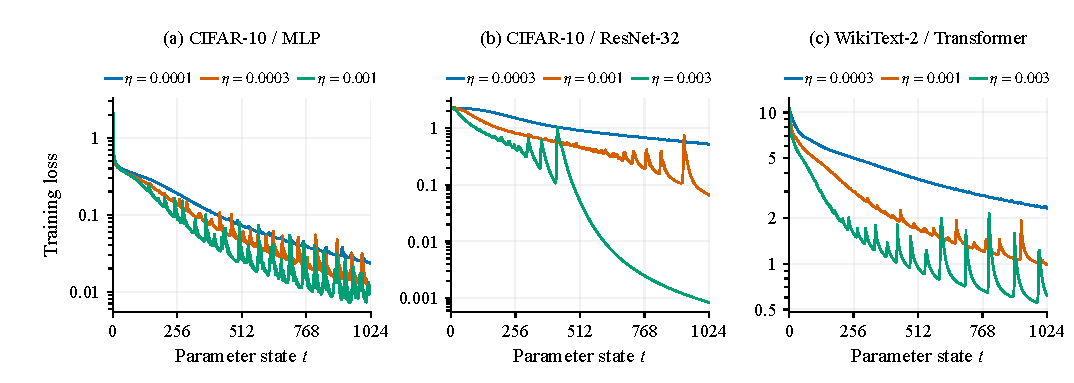
\includegraphics[width=\textwidth]{figures/analysis036/adam_manuscript_overview.pdf}
 \caption{Full-batch Adam training from matched initial weights, with three
 constant learning rates per model. Every training-loss observation is shown
 without smoothing on logarithmic y-axes. Parameter state $s$ denotes $s$
 completed updates, from initialization to 1,024 updates. One initialization
 per model; colors identify increasing rates within each panel.}
 \label{fig:adam-overview}
\end{figure*}


Figure~\ref{fig:adam-overview} shows transient excursions within trajectories
whose longer-term training loss decreases. At 1,024 updates, the largest
tested rate attains the lowest final loss within each model's sweep.
We define the events using loss alone, then describe their population
statistics and individual temporal structure.



\subsection{Loss-Defined Excursions and Their Distribution}



To examine repetition without selecting on gradients, write
$\mathcal L_s:=\mathcal L(\theta_s)$ for the recorded training loss.
Starting at initialization, let $a_i$ be the earliest available state with
$\mathcal L_{a_i+1}>\mathcal L_{a_i}$. Hold the pre-rise reference
$\mathcal L_{a_i}$ fixed. Recovery occurs at the first later state whose
loss is at or below this pre-rise level, $\mathcal L_s\leq\mathcal L_{a_i}$.
For an event recovered within $T$ updates, define
\begin{equation}
\begin{aligned}
 c_i&:=\min\{s:a_i<s\leq T,\ \mathcal L_s\leq\mathcal L_{a_i}\},\\
 p_i&\in\operatorname*{arg\,max}_{a_i<s<c_i}\mathcal L_s.
\end{aligned}
\label{eq:adam-spike-boundaries}
\end{equation}
If several states attain the maximum, $p_i$ is the earliest one.
Figure~\ref{fig:adam-spike-definition} illustrates these boundaries.
An event is included only when recovery is observed by $T=1024$.
Search resumes at $c_i$; partial declines and additional local maxima
before this return belong to the same event. Thus $a_i$ is the last
pre-rise state, $a_i+1$ the first elevated state, $p_i$ the loss peak,
and $c_i$ the first recovered state. Peak increase is
$100(\mathcal L_{p_i}/\mathcal L_{a_i}-1)$; rise and recovery times are
$p_i-a_i$ and $c_i-p_i$, in optimizer updates. The three loss ratios are
$1$, $\mathcal L_{p_i}/\mathcal L_{a_i}$ and
$\mathcal L_{c_i}/\mathcal L_{a_i}\leq1$.



\begin{figure*}[tp]
 \centering
 \begin{minipage}[c]{0.49\textwidth}
 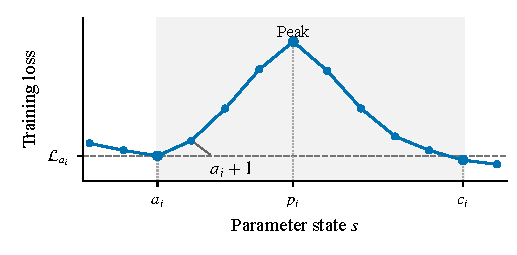
\includegraphics[width=\columnwidth]{figures/analysis036/adam_spike_definition.pdf}
 \end{minipage}\hfill
 \begin{minipage}[c]{0.47\textwidth}
 \caption{Spike boundaries (schematic). The pre-rise state $a_i$ fixes
 the reference loss; $a_i+1$ is the first elevated state, $p_i$ the peak,
 and $c_i$ the first return to or below that reference. Rise and recovery
 durations are $p_i-a_i$ and $c_i-p_i$.}
 \label{fig:adam-spike-definition}
 \end{minipage}
\end{figure*}

\begin{figure*}[tp]
 \centering
 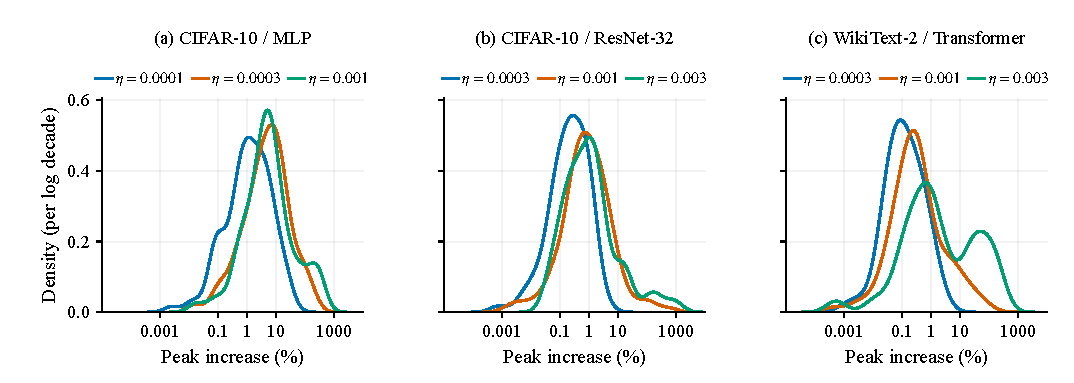
\includegraphics[width=\textwidth]{figures/analysis036/adam_peak_increase_density.pdf}
 \caption{Distributions of peak percentage increases for all 806 recovered
 excursions, including small fluctuations, with no amplitude cutoff.
 Colors identify LRs within each model. Gaussian kernel densities are
 estimated in $\log_{10}$ percentage-increase coordinates with one pooled
 bandwidth per model, common across its LRs. Each LR density integrates
 to one in that coordinate. The log x-axis shows percentage increase:
 1 denotes +1\%, and 100 denotes +100\%. This differs from the loss-ratio
 axis in Fig.~\ref{fig:adam-rho-norm-spikes}.}
 \label{fig:adam-spike-distribution}
\end{figure*}


Figure~\ref{fig:adam-spike-distribution} summarizes all 806 recovered
excursions, including small fluctuations. Larger learning rates populate
more severe excursions, although the distributions overlap and do not
undergo a uniform shift. The densities describe severity conditional on
an observed recovered event; each learning-rate density is normalized
separately and does not represent event frequency.

For the anatomy analysis, we retain events with a peak increase strictly
greater than 10\%. This gives 129 recovered events. Two additional
above-threshold candidates have not recovered by update 1,024 and are
reported separately as unrecovered; the recovery statistics below concern
the recovered sample. Two initialization events have undefined pre-rise
cosine, leaving 127 events for analyses requiring that measurement.
% AUTHOR: Add run-level event counts, event occupancy, absolute loss
% increases, and sensitivity to prespecified thresholds (e.g., 5/10/20%).
% Preserve unrecovered events as censored observations rather than
% silently dropping them from all summaries.
% AUTHOR: Events within one trajectory are not independent replications.
% Add independent initializations and report run-level uncertainty.

\subsection{Amplification and Recovery across Events}

Among qualifying recovered events, both the mean and maximum percentage
increase grow with learning rate in every model with more than one eligible
rate. The largest increase is 858.8\% for ResNet at $\eta=0.003$.
Mean recovery takes 17--19 updates versus 6--8 for the ResNet rise,
and 24--31 versus about 6 for the Transformer. MLP rise and recovery
times are more comparable. A brief amplification can therefore be
followed by a considerably longer return to the pre-rise loss.

Pre-rise raw-gradient cosine is negative in 92.1\% of the events with a
defined measurement. At the loss peak, the gradient norm exceeds its
pre-rise value in every included event. The projected response is above
two before the first loss increase in 16.5\% of defined cases.
Its full-event maximum precedes the loss peak in 63.6\% of events,
coincides in 22.5\%, and follows in 14.0\%. These percentages describe
the phase ordering within the observed events.
% AUTHOR: Report these percentages per run/model as well as pooled.
% The present pooled sample is dominated by the MLP trajectories.
% Compare against ordinary oscillatory windows matched within each run.
% That comparison establishes specificity of the anatomy, not a claim
% that the descriptors constitute an online predictor.



\begin{table*}[tp]
 \caption{Anatomy of recovered spikes with peak increase greater than 10\%.
 Cells report mean $\pm$ sample SD across events; maximum peak increase has
 its own subcolumn. Before denotes a single diagnostic at state $a_i$;
 recovery denotes the event's mean over states $p_i+1,\ldots,c_i$.
 Norm ratios compare loss-peak/pre-rise and recovered/loss-peak endpoints.
 $N$ counts included events; dashes indicate no qualifying event.
 Two initialization events have undefined pre-rise diagnostics, leaving
 46 and 38 observations for those entries in the MLP's middle and highest
 LR rows. No smoothing or averaging across initializations.}
 \label{tab:adam-spike-anatomy}
 \centering
 \footnotesize
 \setlength{\tabcolsep}{1.5pt}
 \renewcommand{\arraystretch}{1.15}
 % Generated by revisions/2026-11-03-regime-writing-revision/01_prepare_table.py.
\begin{tabular*}{\textwidth}{@{\extracolsep{\fill}}*{13}{c}@{}}
\toprule
\multirow{2}{*}{\shortstack{Dataset\\Model}} & \multirow{2}{*}{$\eta$} & \multirow{2}{*}{$N$} & \multicolumn{2}{c}{Peak increase (\%)} & \multicolumn{2}{c}{Time (updates)} & \multicolumn{2}{c}{$\eta\widehat\kappa$ (raw)} & \multicolumn{2}{c}{$\rho$ (raw)} & \multicolumn{2}{c}{Gradient norm ratio} \\
\cmidrule(lr){4-5}\cmidrule(lr){6-7}\cmidrule(lr){8-9}\cmidrule(lr){10-11}\cmidrule(lr){12-13}
 & & & Mean $\pm$ SD & Max & Rise & Recovery & Before & Recovery & Before & Recovery & Rise & Recovery \\
\midrule
\multirow{3}{*}{\shortstack{CIFAR-10\\MLP}} & $10^{-4}$ & 8 & $19\,\mathord{\pm}\,6.1$ & 31 & $8.4\,\mathord{\pm}\,2.9$ & $4.4\,\mathord{\pm}\,2.4$ & $1.8\,\mathord{\pm}\,0.38$ & $1.7\,\mathord{\pm}\,0.08$ & $-0.77\,\mathord{\pm}\,0.31$ & $-0.89\,\mathord{\pm}\,0.08$ & $5.3\,\mathord{\pm}\,1.7$ & $0.30\,\mathord{\pm}\,0.07$ \\
 & $3\times10^{-4}$ & 47 & $43\,\mathord{\pm}\,46$ & 203 & $5.5\,\mathord{\pm}\,4.4$ & $4.9\,\mathord{\pm}\,4.0$ & $1.3\,\mathord{\pm}\,0.25$ & $1.6\,\mathord{\pm}\,0.18$ & $-0.53\,\mathord{\pm}\,0.29$ & $-0.71\,\mathord{\pm}\,0.24$ & $4.5\,\mathord{\pm}\,3.0$ & $0.33\,\mathord{\pm}\,0.13$ \\
 & $10^{-3}$ & 39 & $95\,\mathord{\pm}\,107$ & 318 & $6.1\,\mathord{\pm}\,5.9$ & $7.4\,\mathord{\pm}\,7.5$ & $1.4\,\mathord{\pm}\,0.40$ & $1.4\,\mathord{\pm}\,0.26$ & $-0.46\,\mathord{\pm}\,0.38$ & $-0.55\,\mathord{\pm}\,0.30$ & $5.2\,\mathord{\pm}\,3.8$ & $0.31\,\mathord{\pm}\,0.14$ \\
\midrule
\multirow{3}{*}{\shortstack{CIFAR-10\\ResNet-32}} & $3\times10^{-4}$ & 0 & -- & -- & -- & -- & -- & -- & -- & -- & -- & -- \\
 & $10^{-3}$ & 10 & $105\,\mathord{\pm}\,182$ & 602 & $7.5\,\mathord{\pm}\,2.2$ & $17\,\mathord{\pm}\,11$ & $1.3\,\mathord{\pm}\,0.39$ & $1.3\,\mathord{\pm}\,0.25$ & $-0.36\,\mathord{\pm}\,0.42$ & $-0.36\,\mathord{\pm}\,0.26$ & $4.3\,\mathord{\pm}\,2.9$ & $0.43\,\mathord{\pm}\,0.24$ \\
 & $3\times10^{-3}$ & 7 & $179\,\mathord{\pm}\,309$ & 859 & $6.3\,\mathord{\pm}\,1.3$ & $19\,\mathord{\pm}\,20$ & $1.7\,\mathord{\pm}\,0.38$ & $1.1\,\mathord{\pm}\,0.37$ & $-0.65\,\mathord{\pm}\,0.28$ & $-0.13\,\mathord{\pm}\,0.42$ & $5.0\,\mathord{\pm}\,4.2$ & $0.34\,\mathord{\pm}\,0.24$ \\
\midrule
\multirow{3}{*}{\shortstack{WikiText-2\\Transformer}} & $3\times10^{-4}$ & 0 & -- & -- & -- & -- & -- & -- & -- & -- & -- & -- \\
 & $10^{-3}$ & 6 & $33\,\mathord{\pm}\,25$ & 81 & $6.3\,\mathord{\pm}\,1.9$ & $24\,\mathord{\pm}\,9.8$ & $2.1\,\mathord{\pm}\,0.27$ & $0.96\,\mathord{\pm}\,0.16$ & $-0.84\,\mathord{\pm}\,0.10$ & $-0.02\,\mathord{\pm}\,0.12$ & $9.0\,\mathord{\pm}\,3.8$ & $0.09\,\mathord{\pm}\,0.05$ \\
 & $3\times10^{-3}$ & 12 & $82\,\mathord{\pm}\,70$ & 231 & $6.2\,\mathord{\pm}\,2.7$ & $31\,\mathord{\pm}\,17$ & $2.2\,\mathord{\pm}\,0.43$ & $0.91\,\mathord{\pm}\,0.19$ & $-0.79\,\mathord{\pm}\,0.22$ & $0.09\,\mathord{\pm}\,0.21$ & $11\,\mathord{\pm}\,6.9$ & $0.08\,\mathord{\pm}\,0.08$ \\
\bottomrule
\end{tabular*}

\end{table*}

For Table~\ref{tab:adam-spike-anatomy}, pre-rise diagnostics are measured
at $\theta_{a_i}$, hence use gradient index $a_i+1$. Recovery entries
first average each event's diagnostic over the arrival states
$p_i+1,\ldots,c_i$, then summarize those means across events with equal
event weight. They are not values only at $c_i$. The norm-ratio columns
instead use the endpoints
$\|g_{p_i+1}\|/\|g_{a_i+1}\|$ and
$\|g_{c_i+1}\|/\|g_{p_i+1}\|$. The gradient norm's own maximum need not
coincide with the loss peak.




\paragraph{Individual trajectories.}
For each model, we illustrate the recovered excursion with the largest
peak/pre-rise loss ratio at its highest tested rate. Selection uses
loss alone, with no condition on a gradient diagnostic. The peaks occur
at states 703, 422, and 794 for the MLP, ResNet, and Transformer.



\begin{figure*}[tp]
 \centering
 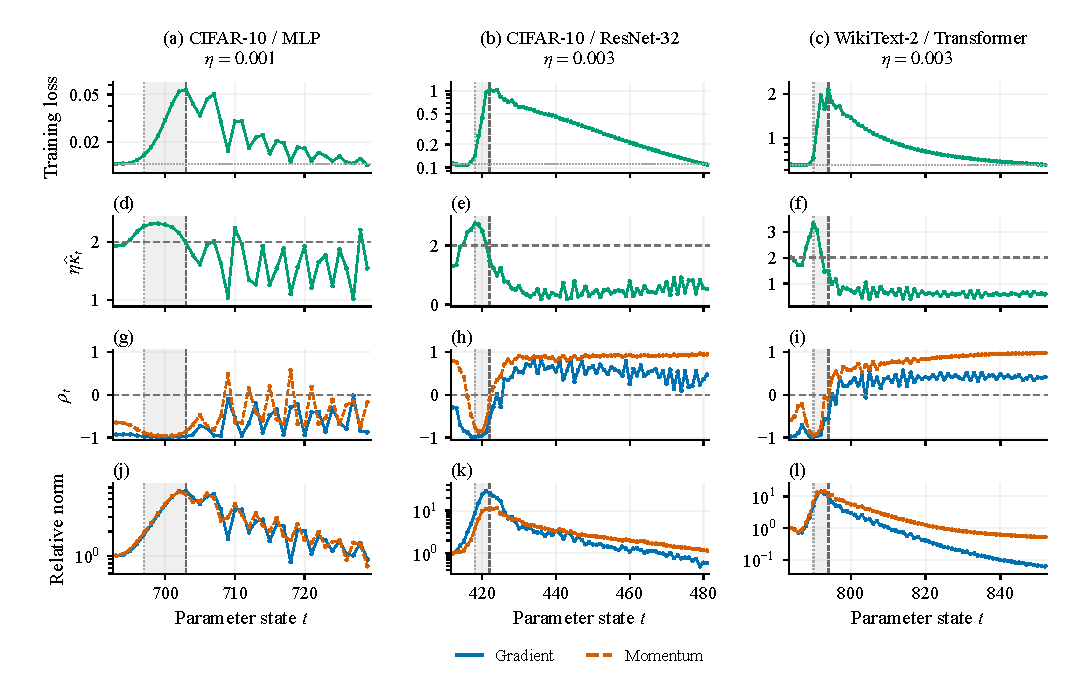
\includegraphics[width=\textwidth]{figures/analysis036/adam_manuscript_spikes.pdf}
 \caption{Largest recovered relative loss spike at each model's highest
 Adam rate. Rows show loss, raw-gradient projected change, consecutive
 cosines of raw gradients and first moments, and their relative norms.
 All observations are unsmoothed. At parameter state $s$, vector diagnostics
 refer to $g_{s+1}$ and $m_{s+1}$. Norms are divided by their value at the
 first displayed state. Gray bands mark the pronounced rise from the first
 +10\% crossing to the loss peak (697--703, 418--422 and 790--794), rather
 than the entire excursion through recovery. The horizontal dotted loss
 reference is the first displayed loss. Windows begin ten states before
 the peak and end at the first later loss below that displayed reference.}
 \label{fig:adam-spikes}
\end{figure*}


All three examples in Fig.~\ref{fig:adam-spikes} enter the pronounced rise
with negative raw-gradient cosine. During the rise, raw-gradient norms
increase sharply, the projected response exceeds two before the loss
maximum, and first-moment norms grow.

Recovery distinguishes the examples. ResNet and Transformer return to
positive raw-gradient and consecutive first-moment alignment, with a
falling projected response and a comparatively smooth loss decline.
The MLP continues to oscillate: its raw-gradient cosine remains mostly
negative, first-moment cosine alternates, and loss and norms decrease
through repeated rebounds. Thus, the illustrations share reversal and
amplification during the rise while exhibiting different recovery
patterns. Population-level phase comparisons are needed to determine
how consistently these patterns recur across initializations.
% AUTHOR: Retain these unsmoothed illustrations, but let aggregate
% event profiles and run-level replication carry broader claims.

\subsection{Alignment and Norm Amplification as Severity Descriptors}

To relate the initial gradient regime to subsequent amplification, define
\begin{equation}
A_i:=\frac{\|g_{p_i+1}\|}{\|g_{a_i+1}\|},
\qquad x_i:=\rho_{a_i+1}A_i,
\label{eq:adam-event-product}
\end{equation}
and compare $x_i$ with the peak/pre-rise loss ratio. The descriptor
combines an initial adjacent-gradient angle with a later norm ratio;
it is a retrospective event summary.



\begin{figure*}[tp]
 \centering
 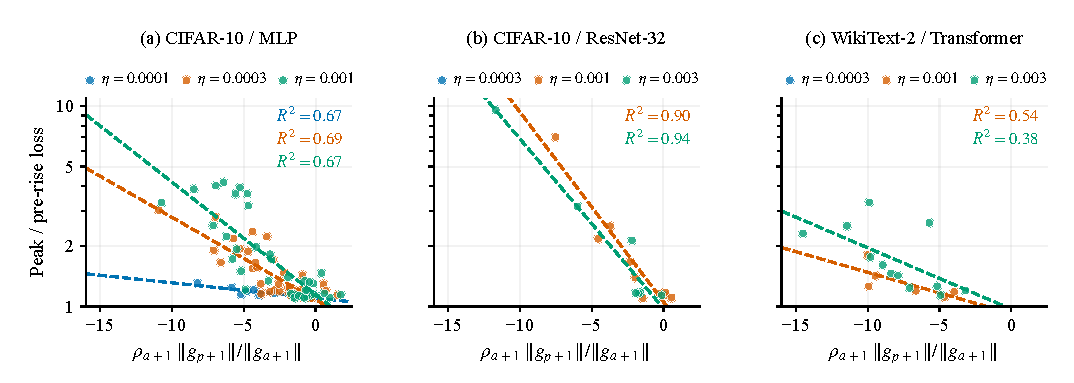
\includegraphics[width=\textwidth]{figures/analysis036/adam_rho_gradient_rise_peak_scatter.pdf}
 \caption{Pre-rise raw-gradient cosine times rise norm ratio versus
 peak/pre-rise loss for 127 recovered spikes above 10\%; two initialization
 events have undefined pre-rise cosine. One unsmoothed point per event.
 Colors identify LRs. Separate per-LR least-squares fits with intercept use
 $\log_{10}$(peak/pre-rise loss) as the response; color-matched $R^2$ values
 are descriptive in-sample scores on that log response. Dashed lines extend
 across each panel, including extrapolation beyond observed samples.
 The y-axis is a loss ratio: 1 denotes no increase and 2 denotes +100\%.}
 \label{fig:adam-rho-norm-spikes}
\end{figure*}


Figure~\ref{fig:adam-rho-norm-spikes} reports separate per-rate fits to
$\log_{10}(\mathcal L_{p_i}/\mathcal L_{a_i})$. Their descriptive,
in-sample $R^2$ values are 0.67--0.69 for the MLP, 0.90--0.94 for ResNet,
and 0.38--0.54 for the Transformer. These associations connect the
individual examples to the event population.

The composite fit does not by itself establish the contribution of
alignment beyond norm amplification. On a fixed one-dimensional quadratic
$\mathcal L(x)=\lambda x^2/2$, the loss ratio equals the squared
gradient-norm ratio exactly. Consequently, norm amplification alone can
explain substantial severity variation even without an additional
alignment effect.
% AUTHOR: Compare cosine-only, norm-only, additive, and interaction
% models with matched transformations and comparable flexibility.
% Include log(A_i) as a natural norm-only baseline. Report sample sizes.
% Assess reproducibility on held-out runs/seeds, not random events from
% the same trajectory. Restrict fitted lines to their observed support.

\subsection{Connecting Gradient Response to Optimizer State}

For a smooth full objective, write
\begin{equation}
P_t:=\operatorname{diag}
\left((\sqrt{\widehat v_t}+\epsilon)^{-1}\right),
\qquad d_t=P_t\widehat m_t,
\end{equation}
and define the starting Hessian $H_t=\nabla^2\mathcal L(\theta_{t-1})$
and its average along the update,
\begin{equation}
\overline H_t:=
\int_0^1\nabla^2\mathcal L(\theta_{t-1}-u\eta d_t)\,du.
\end{equation}
The gradient integral gives
$g_{t+1}-g_t=-\eta\overline H_td_t$, hence
\begin{equation}
\frac{z_{t+1}}{\eta}
=
\frac{g_t^\top\overline H_tP_t\widehat m_t}{\|g_t\|^2}.
\label{eq:adam-response-integral}
\end{equation}
Thus the response reflects both encountered geometry and optimizer state.

With our indexing, the directional quantity of
Bai et al.~\cite{bai2026adaptive} is
\begin{equation}
\begin{aligned}
\lambda_{B,t}
&:=c_t\frac{g_t^\top P_tH_tg_t}{\|g_t\|^2},\\
c_t&:=\frac{1-\beta_1}{(1+\beta_1)(1-\beta_1^t)}.
\end{aligned}
\label{eq:adam-bai-reference}
\end{equation}
Let $e_t:=\widehat m_t-c_tg_t$. Hessian symmetry yields the exact
discrepancy decomposition
\begin{equation}
\begin{aligned}
\frac{z_{t+1}}{\eta}-\lambda_{B,t}
={}&\frac{g_t^\top H_tP_te_t}{\|g_t\|^2}\\
&+\frac{g_t^\top(\overline H_t-H_t)d_t}{\|g_t\|^2}.
\end{aligned}
\label{eq:adam-response-discrepancy}
\end{equation}
The first term measures the effect of departure from the proportional
first-moment response $c_tg_t$. The second measures variation of curvature
along the finite update. This separates the difference between two
diagnostics; causal attribution of spike formation requires additional
controlled experiments.

The first-moment departure is directly connected to adjacent gradient
sums. Let $a=(1-\beta_1)/(1+\beta_1)$ and $r_t=m_t-ag_t$. Substitution
into Eq.~\eqref{eq:adam-moments} gives
\begin{equation}
r_t=\beta_1r_{t-1}+\beta_1a(g_t+g_{t-1}),
\qquad t\ge2,
\label{eq:adam-memory-residual}
\end{equation}
with $e_t=r_t/(1-\beta_1^t)$. The gradient component remaining after
adjacent reversal therefore drives departure from the alternating
first-moment response. For constant-amplitude alternation and a decayed
memory transient, $e_t$ is small. If curvature also varies little along
the update, Eq.~\eqref{eq:adam-response-discrepancy} reduces to
$z_{t+1}\approx\eta\lambda_{B,t}$.

For exact alternation starting at $m_0=0$, the finite-time expression is
$m_t=a[1-(-\beta_1)^t]g_t$; a later alternating segment additionally
inherits its initial memory. Near-opposition alone therefore does not
establish the proportionality when gradient magnitudes or directions
change rapidly.

If the Hessian is $M$-Lipschitz along the step, the discrepancy obeys
\begin{equation}
\begin{aligned}
|z_{t+1}-\eta\lambda_{B,t}|
\leq{}&
\eta\frac{\|H_tg_t\|\,\|P_te_t\|}{\|g_t\|^2}\\
&+\frac{M\eta^2\|d_t\|^2}{2\|g_t\|}.
\end{aligned}
\label{eq:adam-response-error-bound}
\end{equation}
The bound follows from Cauchy--Schwarz and
$\|\overline H_t-H_t\|\leq M\eta\|d_t\|/2$.
It characterizes diagnostic approximation under the stated regularity
conditions; it does not assert a general theorem for the occurrence
or recovery of Adam spikes.
% AUTHOR: Verify the paper's regularity assumptions for each architecture.
% Classical-Hessian identities need qualification at nonsmooth activation
% boundaries; the projected-gradient response itself remains well-defined.
%
% VALIDATION TO ADD (not performed in the supplied experiments):
% 1. Compare z/eta, lambda_B, and lambda_B plus the memory term at selected
%    checkpoints. One HVP H_t*g_t computes both comparison quantities.
% 2. Validate the memory term on rotated anisotropic quadratics; curvature
%    variation vanishes there. beta_1=0 is a useful negative control.
% 3. Hold d_t fixed and evaluate trial steps eta, eta/2, eta/4 to test the
%    finite-step correction at fixed states.
% 4. Compare baseline, refreshed first-moment direction, reference
%    preconditioner, and both changes at matched checkpoints. Include
%    natural and matched step norms. Freeze P or vhat, not merely raw v.
% 5. Test stochastic training using a fixed monitoring objective and
%    occasional same-objective gradient probes; account for their cost.
% 6. If claiming scale, compare instrumentation with the one-HVP baseline
%    and report memory, throughput, communication, precision, and parameter
%    counts consistently. No scale or stochastic validation is claimed here.

\paragraph{Scope of the current empirical findings.}
The full-batch experiments document recovered-excursion anatomy through
changes in the loss slope and first-moment state. The analytic connection
above identifies conditions under which that response approximates a
preconditioned-curvature quantity and specifies sources of discrepancy.
The reported event associations are descriptive. Replication,
ordinary-trajectory controls, and direct measurement of the discrepancy
terms are needed to establish their specificity and practical range.

% Add to the main bibliography:
% @InProceedings{bai2026adaptive,
%   title = {Adaptive Preconditioners Trigger Loss Spikes in {A}dam},
%   author = {Bai, Zhiwei and Zhou, Zhangchen and Zhao, Jiajie and Li, Xiaolong
%     and Li, Zhiyu and Xiong, Feiyu and Yang, Hongkang and Zhang, Yaoyu
%     and Xu, Zhi-Qin John},
%   booktitle = {Proceedings of the 43rd International Conference on Machine Learning},
%   pages = {5566--5601},
%   year = {2026},
%   volume = {306},
%   series = {Proceedings of Machine Learning Research},
%   publisher = {PMLR},
%   url = {https://proceedings.mlr.press/v306/bai26o.html}
% }

